\chapter{Full parameter table}
\label{app:parameters}
\section*{Iterative density-peak discovery}
Within each random group of about \num{30000} frames, discovery proceeds as follows.
\begin{protocolsteps}
\item \textbf{Generate candidates.} Start discovery at $d_c=1.3$, rank candidate centres by $\rho_i\delta_i$, and try 10 down to 2 centres.
\item \textbf{Check each cluster.} Require at least 300 members and a mean silhouette of at least 0.3 for acceptance.
\item \textbf{Choose the candidate.} Keep the one with the most acceptable clusters. A tie retains the earlier, higher-centre-count candidate.
\item \textbf{Continue on the remainder.} Remove accepted members and multiply $d_c$ by 0.9 before the next iteration.
\item \textbf{Stop discovery.} Stop below 300 remaining points or after five consecutive unsuccessful iterations. Residual frames receive their final labels only in STEP~3.
\end{protocolsteps}

\begingroup\small
\begin{longtable}{@{}>{\raggedright\arraybackslash}p{.34\textwidth}>{\raggedright\arraybackslash}p{.22\textwidth}>{\raggedright\arraybackslash}p{.36\textwidth}@{}}
\caption{Reproduction settings and execution profiles. These parameters are implemented but do not imply a completed empirical run.}\label{tab:parameters}\\
\toprule Parameter & Value & Evidence / role\\\midrule\endfirsthead
\multicolumn{3}{l}{\small\itshape Table \thetable\ continued}\\
\toprule Parameter & Value & Evidence / role\\\midrule\endhead
Replicas & 3 & Primary paper; observed table segmentation\\
Analysis interval & 1--3 μs & Published baseline; inclusive source-labelled ps boundaries\\
Temperature & 310 K & Published weighting parameter; no new MD run\\
Bias factor $\gamma$ & 10 & Published weighting parameter\\
Molar gas constant & 0.008314462618 kJ mol$^{-1}$ K$^{-1}$ & Implementation unit convention\\
CV conversions & $\alpha=\na/1.1$, $\beta=\nb/2.5$ & Published descriptor scaling\\
Baseline features & $\na$, $\nb$, $R_g$, SASA & Pooled min--max normalization\\
Initial $d_c$ & 1.3 & Published baseline\\
Cutoff multiplier & 0.9 & Published 10\% reduction\\
Center-count scan & 10 down to 2 & Published baseline\\
Minimum cluster size & 300 frames & Published acceptance criterion\\
Minimum mean silhouette & 0.3 & Published acceptance criterion\\
Failure stopping count & 5 & Consecutive iterations with no accepted cluster\\
Distance storage & float32 & Source-informed; blockwise construction\\
Consensus & Average linkage & Marginal Wasserstein norm\\
Elbow smoothing & $s=5$ & Supplied source heuristic\\
Elbow search range & First 90\% of merges & Supplied source heuristic\\
Final assignment & One nearest-centroid pass & No iterative refitting\\
Master seed & 42 & Default project configuration; recorded per run\\
Smoke / medium groups & 3,000 / 10,000 & Reduced execution profiles\\
Smoke / medium discovery groups & 2 / 3 & Not full-production evidence\\
Full group size & About 30,000 & All groups; full execution disabled\\
Seed counts & 2 smoke; 5 pilot/medium; 20 full default & Full robustness configurable; not performed\\
Bootstrap draws & 500 & Conditional moving-block extension; not performed on real weights\\
Resource policy & Bounded sequential local workers & Full execution held for review\\
\bottomrule
\end{longtable}
\endgroup
\addsec{Completed descriptor-only GMM pilot}
The protocol was committed before execution. Its four operations separate the choice of fitting observations from the comparisons made afterwards:
\begin{protocolsteps}
\item \textbf{Fix the sample.} Select 1,000 frames per replica with seed 20261007. Use the same 3,000 observations for every fit.
\item \textbf{Fit the transformation.} Estimate means and population standard deviations on those rows only. Share the transformation of retained descriptors between the four- and three-feature representations.
\item \textbf{Fit the models.} For each $K=2,\ldots,6$, use seeds 42--46: 50 fits overall. Each fit uses one initialization, at most 500 iterations, tolerance $10^{-3}$ and covariance regularization $10^{-6}$.
\item \textbf{Compare assignments.} Label all 300,003 frames, including fitting rows. Use five paired-seed ARIs to compare representations and ten seed pairs to compare initializations within each representation.
\end{protocolsteps}

The following settings belong to the successful independent experiment, not to the published DPC baseline. The fit sample and initializations were recorded before execution.
\begin{longtable}{@{}>{\raggedright\arraybackslash}p{.34\textwidth}>{\raggedright\arraybackslash}p{.22\textwidth}>{\raggedright\arraybackslash}p{.36\textwidth}@{}}
\caption{Settings of the completed GMM experiment, as recorded in its run manifest.}\label{tab:gmmparameters}\\
\toprule Parameter & Value & Evidence / role\\\midrule\endfirsthead
\multicolumn{3}{l}{\small\itshape Table \thetable\ continued}\\
\toprule Parameter & Value & Evidence / role\\\midrule\endhead
Fit sample & 1,000 per replica & 3,000 rows; shared across models\\
Sampling seed & 20261007 & Local NumPy generator\\
Feature spaces & Four descriptors; omit SASA & Same scaling for shared features\\
Scaling & Fit-sample mean and SD & No evaluation-data refit\\
Components & 2, 3, 4, 5, 6 & All counts retained in comparison\\
Initialization seeds & 42, 43, 44, 45, 46 & Paired across representations\\
Initializations per fit & 1 & 50 total fitted models\\
Covariance & Full & Regularization $10^{-6}$\\
Convergence settings & 500 iterations; tolerance $10^{-3}$ & All fits converged numerically\\
Evaluation & 300,003 rows & Includes fit rows; descriptive comparison\\
Resource limits & 600 s; 4 GiB & Sequential local worker\\
\bottomrule
\end{longtable}

\chapter{Mathematical derivations and estimator checks}
\label{app:derivations}
\section*{Gaussian hills and bias construction}
The accumulated potential can be written as a sum of local Gaussian hills:
\begin{equation}
V(s,t)=\sum_{t_k<t}h_k\exp\!\left[-\frac12\sum_a\frac{(s_a-s_a(t_k))^2}{\sigma_a^2}\right].
\label{eq:hills}
\end{equation}
In \cref{eq:hills}, $s$ is the CV vector, $t_k$ a deposition time, $h_k$ the hill height and $\sigma_a$ its width along coordinate $a$. Well-tempered heights follow $h_k=h_0\exp[-V(s(t_k),t_k)/(k_B\Delta T)]$ in molecular energy units; molar units require $R$ instead of $k_B$.

\section*{Why the sign of the final-bias correction is negative in FES form}
Under a static bias $V$, the observed configuration density is proportional to $\exp[-\beta_T(U+V)]$. Multiplying by $\exp(\beta_T V)$ recovers relative canonical density. The WT relation $V\simeq-(1-1/\gamma)F+C$ therefore gives the negative free-energy sign in \cref{eq:finalweights}. Applying $\exp(-\beta_T V)$ would reverse the correction. This derivation assumes that using a final bias is appropriate for the analyzed interval; it is not a proof that the supplied trajectories satisfy that assumption.

\section*{Kish effective sample size}
Unequal statistical weights require a separate diagnostic:
\begin{equation}
N_{\mathrm{eff,Kish}}=\frac{(\sum_i w_i)^2}{\sum_i w_i^2}.
\label{eq:kish}
\end{equation}
\Cref{eq:kish} measures weight concentration without correcting temporal dependence. It is not automatically combined with correlation ESS. No empirical Kish ESS is available without validated weights.

\section*{Equal-replica mixture and cluster moments}
Let $\widetilde w_{ri}$ sum to one within replica $r$. The pooled expectation of $A$ is $(1/3)\sum_r\sum_i\widetilde w_{ri}A_{ri}$. Cluster relevance uses $A$ equal to a membership indicator. For a conditional cluster mean, divide the pooled weighted sum of the descriptor by the pooled membership mass. Computing three conditional means and averaging them equally instead would answer a different question when cluster populations differ across replicas.

\section*{Bilinear interpolation test}
For a cell with fractional coordinates $u,v\in[0,1]$, interpolation combines its four corner values with weights $(1-u)(1-v)$, $u(1-v)$, $(1-u)v$, and $uv$. Their sum is one. Any surface $a+b\alpha+c\beta+d\alpha\beta$ is reproduced exactly within floating-point tolerance. The test suite includes such a mixed-term surface, reordered input rows, boundaries and invalid-grid cases, providing stronger evidence than checking a single grid node.

\chapter{Additional diagnostics and interpretation}
\label{app:diagnostics}
\begin{figure}[!htbp]
\centering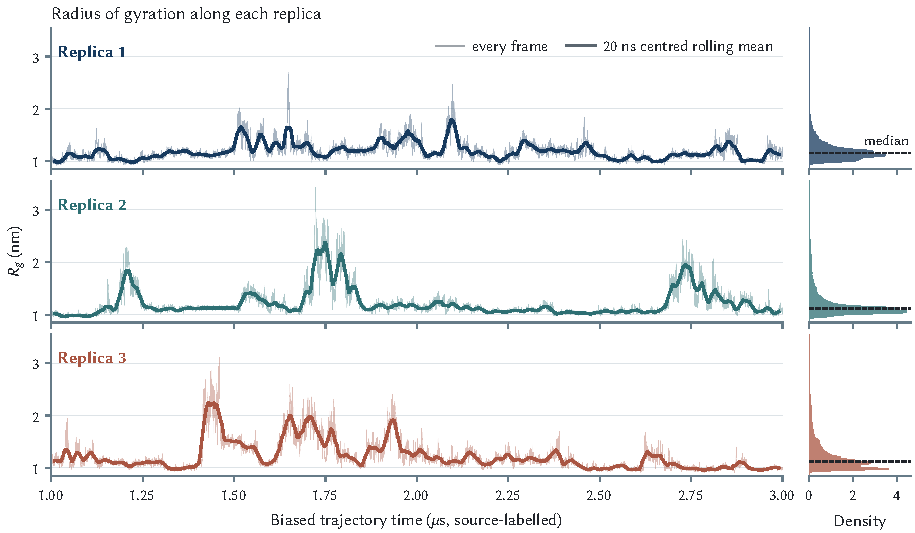
\includegraphics[width=\textwidth]{rg_timeseries.pdf}
\caption{Radius of gyration along the biased trajectory of each replica. Thin lines show every frame and bold lines a centred 20 ns (1,000-frame) rolling mean. The right-hand histograms are unweighted densities with dashed lines at the medians (1.153, 1.118 and 1.126 nm).}
\label{fig:rgtrace}
\end{figure}
\begin{table}[htbp]
\centering
\begin{threeparttable}
\caption{Agreement between feature sets across the five paired initializations.}
\label{tab:gmm}
\begin{tabular}{@{}crr@{}}\toprule Components & Median ablation ARI & Observed range\\\midrule
2 & 0.690 & 0.188--0.868 \\
3 & 0.864 & 0.862--0.868 \\
4 & 0.607 & 0.548--0.622 \\
5 & 0.531 & 0.382--0.696 \\
6 & 0.457 & 0.294--0.461 \\
\bottomrule\end{tabular}

\begin{tablenotes}[flushleft]\footnotesize
\item Component counts were specified for comparison, not selected as physical numbers of states.
\end{tablenotes}
\end{threeparttable}
\end{table}
\begin{figure}[!htbp]
\centering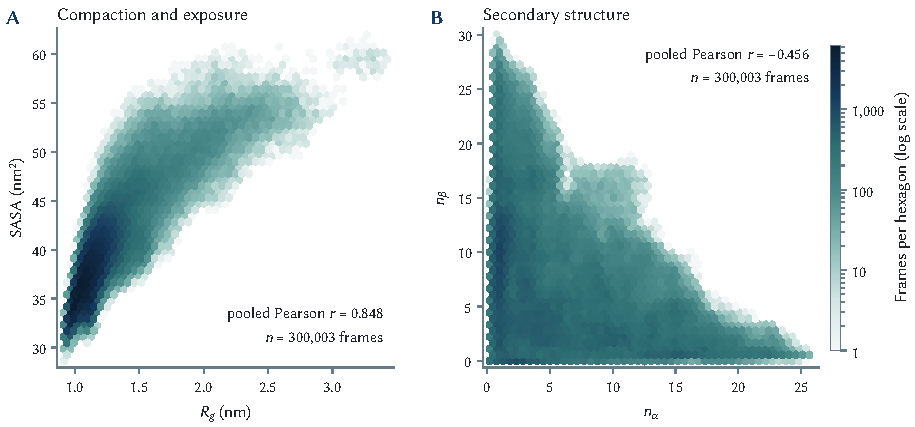
\includegraphics[width=\textwidth]{descriptor_landscape.pdf}
\caption{Unweighted descriptor landscape of the pooled sample (300,003 frames, three replicas, 1--3 μs). (A) Radius of gyration against SASA. (B) $\na$ against $\nb$. Shading is the log number of frames per hexagonal cell on a shared scale.}
\label{fig:landscape}
\end{figure}
\begin{figure}[!htbp]
\centering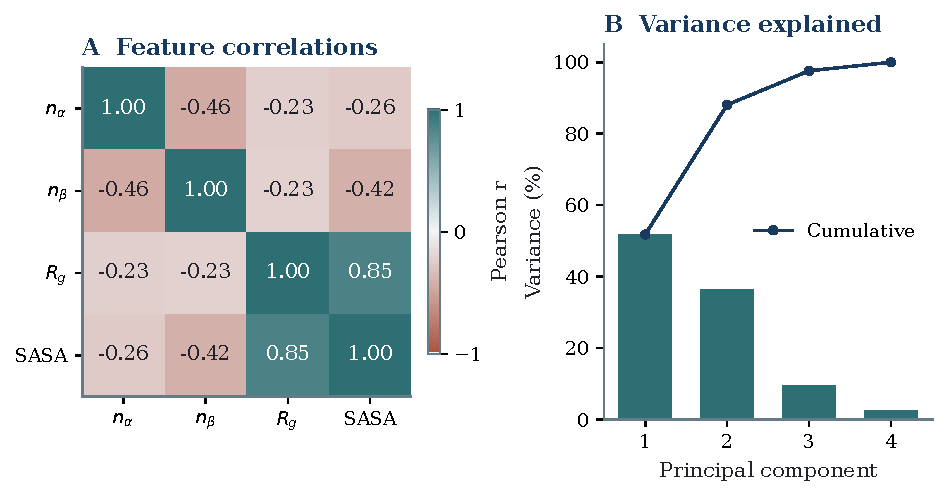
\includegraphics[width=\textwidth]{rebuild_features.pdf}
\caption{Relationships between the four descriptors in the pooled, unweighted sample. Left: Pearson correlation matrix. Right: variance explained by standardized PCA, with cumulative variance shown by the line.}
\label{fig:features}
\end{figure}
\begin{figure}[!htbp]
\centering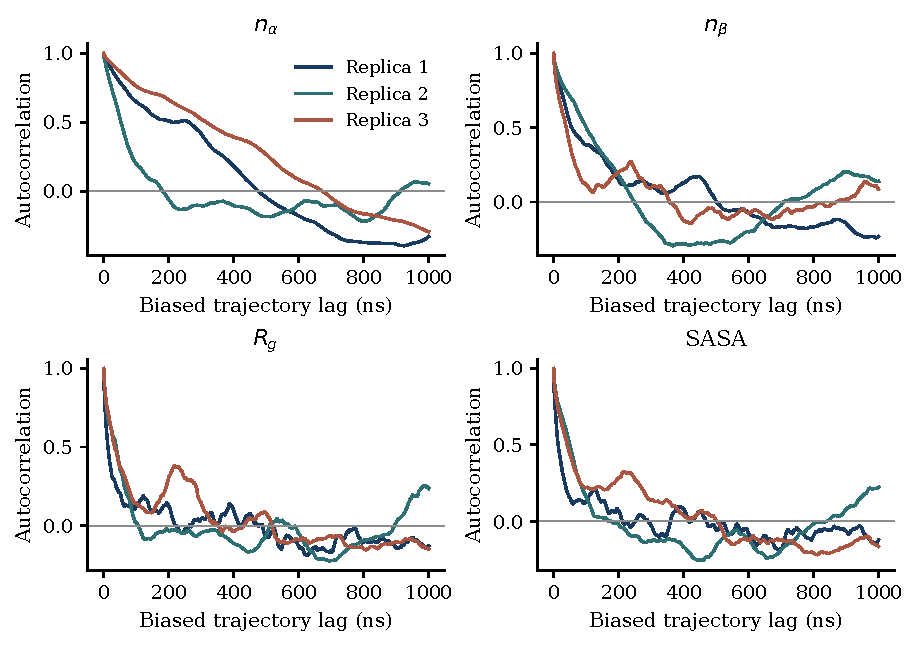
\includegraphics[width=.95\textwidth]{rebuild_autocorrelations.pdf}
\caption{Autocorrelation functions calculated separately for each replica and descriptor. For readability the figure displays a subset of lag points over the first half of the available window; estimation uses the full ACF sequence. The horizontal axis is biased trajectory time.}
\label{fig:acf}
\end{figure}

\begin{figure}[htbp]
\centering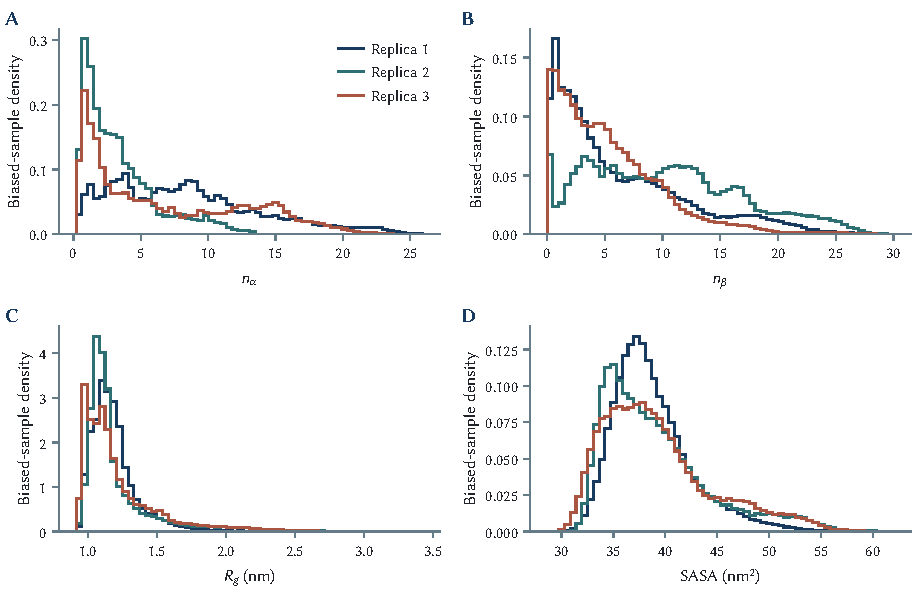
\includegraphics[width=\textwidth]{raw_descriptor_distributions.pdf}
\caption{Per-replica distributions of the recorded descriptors. Each descriptor uses common bin edges, with separate density normalization for each replica. The curves retain the simulation bias and are not equilibrium distributions. Units follow the source labels.}
\label{fig:rawdistributions}
\end{figure}
\begin{table}[htbp]
\centering
\caption{All recorded correlation estimates, each flagged as unreliable by at least one stated check. $g$ denotes statistical inefficiency. The half-window shift is the absolute difference of means divided by the full-series standard deviation. The time axis belongs to the biased trajectory.}
\label{tab:sampling}\small
\begin{tabular}{@{}clrrrr@{}}\toprule
Replica & Descriptor & $g$ & $\tau_{\mathrm{int}}$ (ns) & $N_{\mathrm{eff,corr}}$ & Half shift / SD\\\midrule
1 & $n_\alpha$ & 22067 & 220.7 & 4.5 & 1.28 \\
1 & $n_\beta$ & 11079 & 110.8 & 9.0 & 0.83 \\
1 & $R_g$ & 3679 & 36.8 & 27.2 & 0.27 \\
1 & SASA & 3490 & 34.9 & 28.7 & 0.36 \\
2 & $n_\alpha$ & 6259 & 62.6 & 16.0 & 0.37 \\
2 & $n_\beta$ & 10843 & 108.4 & 9.2 & 0.41 \\
2 & $R_g$ & 3951 & 39.5 & 25.3 & 0.33 \\
2 & SASA & 5325 & 53.2 & 18.8 & 0.17 \\
3 & $n_\alpha$ & 31742 & 317.4 & 3.2 & 1.61 \\
3 & $n_\beta$ & 5880 & 58.8 & 17.0 & 0.71 \\
3 & $R_g$ & 6259 & 62.6 & 16.0 & 0.88 \\
3 & SASA & 9958 & 99.6 & 10.0 & 0.87 \\
\bottomrule\end{tabular}

\end{table}
The saved tables contain per-replica raw descriptor counts, means, standard deviations, extrema, common-bin histograms, the full four-feature correlation matrix, PCA transformation parameters and explained variance, and the reported correlation-estimator diagnostics. The ACF figure is a plotting subsample, not the series used to estimate $g$. No weights are present in these real-data diagnostic summaries.

The half-window mean-shift diagnostic is descriptive. A large shift can arise from slow fluctuations, nonstationarity, or changing occupation of sampled regions. Its threshold is an explicit project heuristic. A low shift alone would not establish convergence, and no threshold outcome can recover an unbiased time scale from WT-MetaD time. Future evaluation should preserve these distinctions when adding weighted estimates.

\begin{figure}[htbp]
\centering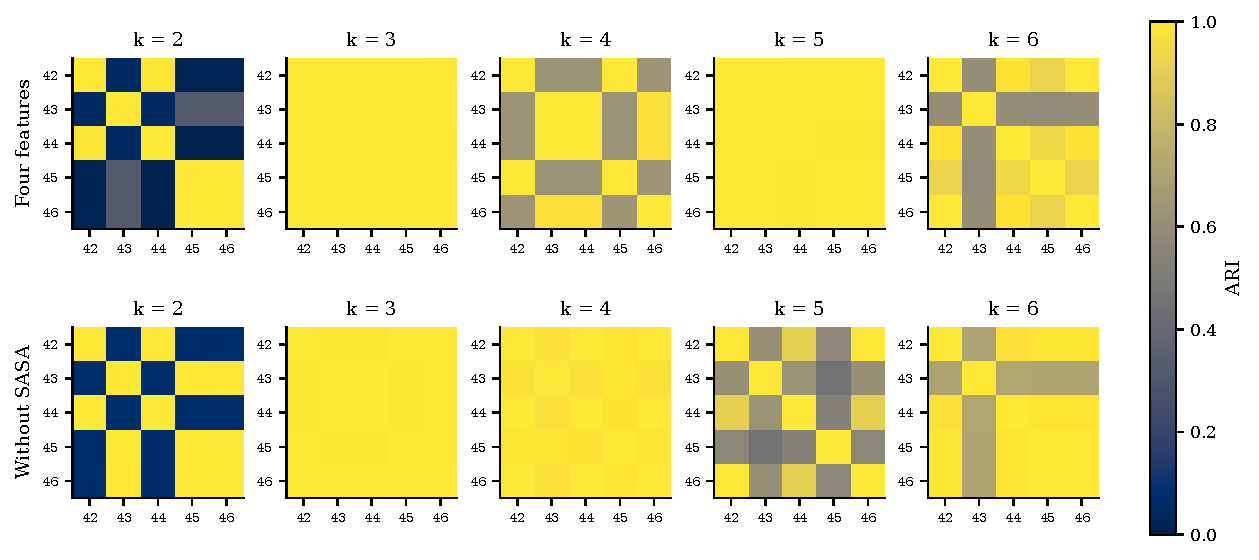
\includegraphics[width=\textwidth]{gmm_seed_matrices.pdf}
\caption{All pairwise seed ARIs from the GMM pilot. Columns show each tested component count; rows distinguish the four-feature and SASA-ablated representations. The diagonal is identity. All fits converged, so no entries are omitted. Similar numerical stopping status can coexist with different partitions.}
\label{fig:seedmatrices}
\end{figure}

\chapter{Code audit summary}
\label{app:codeaudit}
\begin{figure}[htbp]
\centering% Layered architecture of the robustcluster-abeta package (v0.3.0), drawn from the source tree:
% src/robustcluster_abeta/*.py imports, pyproject [project.scripts], config/*.yaml, workflows/Snakefile,
% scripts/, tests/ (36 tests passed in results/logs/*/pytest.log) and .github/workflows/ci.yml.
% gmm_ablation.py is called by cli.py directly (not by pipeline.py) and reads descriptors through io.py
% with its own scaler, so it receives no arrow from preprocessing.py.
% Solid frame: implemented and tested. Dashed frame: implemented; depends on the FES unit, run under the assumption stated in the report.
% Native TikZ; needs only arrows.meta (already loaded by preamble.tex).
\begin{tikzpicture}[
  font=\sffamily\footnotesize,
  every node/.append style={execute at begin node={\hyphenpenalty=10000\exhyphenpenalty=10000}},
  box/.style={draw=Navy!55,fill=CoolGrey,line width=.5pt,rounded corners=1.2pt,
    text width=#1,minimum height=10mm,align=center,inner sep=2.4pt,text=Ink,
    font=\sffamily\scriptsize},
  box/.default=27.2mm,
  pending/.style={box=#1,dashed,fill=white,draw=Navy!45},
  outbox/.style={box=#1,fill=Navy,draw=Navy,text=white},
  outbox/.default=27.2mm,
  frame/.style={draw=Teal!70,line width=.5pt,rounded corners=2pt,fill=Teal!6},
  flow/.style={-{Stealth[length=4.5pt,width=4pt]},draw=Navy!70,line width=.6pt},
  lane/.style={font=\sffamily\scriptsize\bfseries\addfontfeatures{LetterSpace=8},
    text=Teal,anchor=east},
  lanetop/.style={font=\sffamily\scriptsize\bfseries\addfontfeatures{LetterSpace=8},
    text=Teal,anchor=south}]
\def\ttl#1{{\footnotesize\bfseries #1}\\}
% main stack: columns centred at 15, 49, 83 mm (outer width 32 mm); right lane centred at 117 mm
% ---------------- INPUT
\node[box] (desc) at (15mm,0)  {\ttl{descriptor table}data/raw/\\{\fontsize{7.2}{8.6}\selectfont input\_clustering\_ab40.dat}};
\node[box] (fesin) at (49mm,0) {\ttl{FES grid}data/raw/\\FES\_AB\_40.dat};
\node[box] (yaml) at (83mm,0)  {\ttl{YAML config}config/*.yaml\\three run profiles};
% ---------------- I/O
\node[box] (io)  at (15mm,-15mm) {\ttl{io.py}read descriptors, check replicas};
\node[box] (fes) at (49mm,-15mm) {\ttl{fes.py}audit\_fes.py: grid structure, units};
\node[box] (man) at (83mm,-15mm) {\ttl{manifest.py}load config; hashes, run record};
\draw[flow] (desc) -- (io);  \draw[flow] (fesin) -- (fes);  \draw[flow] (yaml) -- (man);
% shared validation bar
\node[box=95.2mm,minimum height=5.5mm,fill=white,draw=Navy!40] (val) at (49mm,-25.5mm)
  {\textbf{validation.py} \textperiodcentered{} finite checks, time and memory budget, blocked vs failed states};
\draw[flow] (io) -- (io |- val.north);  \draw[flow] (fes) -- (fes |- val.north);
\draw[flow] (man) -- (man |- val.north);
% ---------------- SCALING
\node[box=95.2mm,minimum height=8mm] (pre) at (49mm,-35mm)
  {\ttl{preprocessing.py}min--max scaling of the four features \textperiodcentered{} random disjoint frame groups};
\draw[flow] (val) -- (pre);
% ---------------- ANALYSIS
\draw[frame] (0,-43mm) rectangle (72mm,-80mm);
\node[anchor=north west,inner sep=0pt,font=\sffamily\scriptsize,text=Teal] at (1.6mm,-44.3mm)
  {\textbf{pipeline.py} \textperiodcentered{} orchestrates the analysis stages};
\draw[flow] (36mm,-39mm) -- (36mm,-43mm);
\begin{scope}[every node/.append style={minimum height=12.5mm}]
  \node[box=19.4mm] (dpc)  at (12.3mm,-56mm) {\ttl{dpc.py}iterative density-peak clustering};
  \node[box=19.4mm] (con)  at (36mm,-56mm)   {\ttl{consensus.py}Wasserstein merge, frame assignment};
  \node[box=19.4mm] (stab) at (59.7mm,-56mm) {\ttl{stability.py}ARI, partition matching};
  \node[box=19.4mm] (stat) at (12.3mm,-71mm) {\ttl{statistics.py}ACF, Kish ESS, block bootstrap};
  \node[pending=43.1mm] (rw) at (47.85mm,-71mm) {\ttl{reweighting.py}FES-derived frame weights,\\equal-replica normalization};
  \node[box=22.4mm] (gmm) at (86.8mm,-71mm) {{\scriptsize\bfseries gmm\_ablation.py}\\Gaussian-mixture ablation, descriptor-only};
\end{scope}
\draw[flow] (dpc) -- (con);
% ---------------- OUTPUT
\node[box] (mf)  at (15mm,-92mm) {\ttl{results/manifests/}JSON run manifests};
\node[box] (tab) at (49mm,-92mm) {\ttl{results/tables/}CSV summaries};
\node[box] (fig) at (83mm,-92mm) {\ttl{plotting.py}figure scripts \textrightarrow{} results/figures/};
\draw[flow] (15mm,-80mm) -- (mf);
\draw[flow] (49mm,-80mm) -- (tab);
\draw[flow] (gmm.south) -- (gmm.south |- fig.north);
\draw[flow] (tab) -- (fig);
% ---------------- REPORT
\node[box] (prep) at (15mm,-107mm) {\ttl{prepare\_report.py}report/generated/*.tex};
\node[box] (bld)  at (49mm,-107mm) {\ttl{build\_report.py}latexmk \textperiodcentered{} LuaLaTeX};
\node[outbox] (pdf) at (83mm,-107mm) {\ttl{report.pdf}this report};
\draw[flow] (mf) -- (prep);
\draw[flow] (prep) -- (bld);  \draw[flow] (bld) -- (pdf);
\draw[flow] (fig.south) -- ++(0,-2.5mm) -| ([xshift=6mm]bld.north);
% ---------------- left lane labels
\foreach \y/\t in {0/INPUT,-15/{I/O},-25.5/CHECKS,-35/SCALING,-61.5/ANALYSIS,-92/OUTPUT,-107/REPORT}
  \node[lane] at (-2.5mm,\y mm) {\t};
% ---------------- right lane: entry points, tests and CI
\node[lanetop] at (117mm,-8mm) {ENTRY};
\node[box=23.2mm] (snk) at (117mm,-15mm) {\ttl{Snakefile}workflows/, via workflow\_stage.py};
\node[box=23.2mm,minimum height=12.5mm] (cli) at (117mm,-56mm) {\ttl{cli.py}console script robustcluster, seven commands};
\draw[flow] (snk) -- (cli);
\draw[flow] (cli) -- (72mm,-56mm);
\draw[flow] (cli.south) |- (gmm.east);
\node[lanetop] at (117mm,-85mm) {QUALITY};
\node[box=23.2mm] (tst) at (117mm,-92mm) {\ttl{tests/}38 pytest tests};
\node[box=23.2mm] (ci) at (117mm,-107mm) {\ttl{GitHub Actions}ruff + pytest, Python 3.12};
\draw[flow] (ci) -- (tst);
% ---------------- legend
\node[anchor=north,font=\sffamily\scriptsize,text=Ink] at (55mm,-115mm)
  {\tikz[baseline=-.6ex]\draw[Navy!55,fill=CoolGrey] (0,-1.2mm) rectangle (4.5mm,1.2mm);\enspace implemented and tested\qquad
   \tikz[baseline=-.6ex]\draw[Navy!45,dashed] (0,-1.2mm) rectangle (4.5mm,1.2mm);\enspace depends on the FES unit\qquad
   \tikz[baseline=-.6ex]\draw[Teal!70,fill=Teal!6] (0,-1.2mm) rectangle (4.5mm,1.2mm);\enspace called by pipeline.py};
\end{tikzpicture}

\caption{Architecture of the \code{robustcluster-abeta} package. Inputs pass through validation and scaling to the analysis modules orchestrated by \code{pipeline.py}; results go to manifest-backed tables and figures and then into this report. \code{gmm\_ablation.py} is the separate descriptor-only experiment of \cref{sec:task3}. The dashed module depends on the FES unit and was run under the assumption of \cref{sec:weighted}.}
\label{fig:architecture}
\end{figure}
\section*{Two numerical tests}
Two small examples from the 38-test suite show how a check can identify a numerical error without relying on the output of the full pipeline.

\paragraph{Interpolation with a known answer.}
An analytic bilinear surface includes a mixed-coordinate term, so a query between nodes tests both axes together. Reordering its rows must preserve the interpolated answer. Deleting or duplicating a grid point, or querying outside the bounds, must instead raise an error. The same fixture therefore checks both a valid calculation and the rejection of inputs for which that calculation would be inappropriate.

\paragraph{Normalization with an invariant.}
An arbitrary additive FES constant must disappear after weight normalization. A second check gives two replicas unequal numbers of frames and requires each to contribute half of the pooled mass. This catches pooling by row count, which would look correct on three equal-length replicas. Other weight tests check the formula's sign and weighted moments.

The remaining checks cover parsing, scaling, residual exclusion and final assignment. Renaming cluster labels must leave partition agreement unchanged; changing evaluation extremes must not alter a scaler fitted on fixed training rows. These checks isolate failures that could otherwise be mistaken for a change in the clustering method.

A synthetic end-to-end fixture exercises discovery, consensus, weighting, summaries and figure generation. Synthetic GMM cases check repeatability and missing-family handling. An autoregressive fixture probes the correlation estimator; an archive test prevents an unrelated enclosing Git repository from supplying false provenance. The fixtures establish software behaviour on known inputs (Scope~5).

The project inventory records immutable source hashes, table dimensions and missing inputs. The method map links each step to paper evidence, source behavior, the modular implementation and validation tests. The decision log records scientific category and expected effect. The open-questions register prevents uncertain provenance from being converted into hidden defaults.

Scientific V2 is absent, so the audit contains no invented intermediate diff. The supplied original remains excluded from execution and lint collection because its syntax error and top-level writes are part of the preserved evidence. New code is tested independently. Public source packaging excludes the raw table and original script until their redistribution rights are established.



The checked bibliography contains journal articles and official documentation records; its matrix links each citation to its question, method, relevance, and report section. Online-first dates and issue years are distinguished. References whose publisher verification remained unresolved are documented outside the BibTeX file rather than filled from memory.

\chapter{Reproducibility instructions and software environment}
\label{app:repro}
The project source, tests, configurations and this report are available at
\href{https://github.com/Alierkn/robustcluster-abeta}{RobustCluster-Aβ on GitHub}.
The \href{https://github.com/Alierkn/robustcluster-abeta/tree/main/src/robustcluster_abeta}{Python package}
and \href{https://github.com/Alierkn/robustcluster-abeta/tree/main/report}{LaTeX sources}
can be inspected separately or downloaded together using GitHub's \textit{Code / Download ZIP} option.
The repository guide distinguishes code verification and report regeneration from analyses requiring restricted inputs.

\begin{lstlisting}
python3.12 -m venv .venv
source .venv/bin/activate
python -m pip install -r requirements-lock.txt
python -m pip install --no-deps -e .
pytest -q
ruff check src tests scripts
robustcluster validate --config config/paper_reproduction.yaml
robustcluster diagnostics --config config/robustness.yaml
robustcluster cluster --config config/paper_reproduction_full.yaml --profile full
robustcluster reproduce --config config/paper_reproduction_full_assumed.yaml --profile full
\end{lstlisting}
The raw file must first be obtained and checked against its documented SHA256. The standalone commands and Snakemake workflow use the same package functions. The report imports successful diagnostics, FES-audit, GMM and figure manifests with matching hashes. Its generated editorial artwork and real browser screenshots have separate provenance records. LuaLaTeX, Biber and latexmk build the supplied report sources; current paths and tool versions are recorded in the build manifest.

The full-profile configurations record the measured resource estimates that justified enabling them (about 15 minutes and 4~GiB per clustering run). The configuration with the assumed FES unit states that assumption in its header and in every manifest it produces; once the unit is confirmed, only its two FES fields need to change. Outputs that would redistribute the FES or per-frame descriptor values stay local, with their hashes kept in the manifests. No calculation in this report used an HPC system \autocite{leonardodocs}.

\addsec{Software environment}
\begin{table}[htbp]
\centering
\begin{threeparttable}
\caption{Software versions for the reported local descriptor diagnostics.}
\label{tab:environment}
\begin{tabular}{@{}ll@{}}\toprule Component & Version in diagnostic manifest\\\midrule
Python & 3.12.6 \\
numpy & 2.5.3 \\
scipy & 1.18.1 \\
scikit-learn & 1.9.1 \\
pandas & 2.3.3 \\
matplotlib & 3.11.2 \\
robustcluster-abeta & 0.1.0 \\
\bottomrule\end{tabular}

\begin{tablenotes}[flushleft]\footnotesize
\item The GMM pilot manifest records the same versions. They do not describe the original authors' simulation environment. The complete dependency lock and report-tool versions are separate reproducibility artifacts.
\end{tablenotes}
\end{threeparttable}
\end{table}

\chapter{Personal projects and source-code evidence}\label{app:companion}
\begin{figure}[htbp]
\centering% Tooling map: where the student's tools sit relative to the analysis in this report.
% MCP projects labelled from the READMEs of github.com/Alierkn/vmd-mcp and github.com/Alierkn/gromacs-mcp.
% Dashed frame: personal project, not used to produce the supplied Abeta40 data.
% Native TikZ; needs only arrows.meta (already loaded by preamble.tex). Uses \abforty from preamble.tex.
\begin{tikzpicture}[
  font=\sffamily\footnotesize,
  every node/.append style={execute at begin node={\hyphenpenalty=10000\exhyphenpenalty=10000}},
  tool/.style={draw=Navy!55,fill=CoolGrey,line width=.5pt,rounded corners=1.2pt,
    text width=35mm,minimum height=14mm,align=center,inner sep=3pt,text=Ink,
    font=\sffamily\scriptsize},
  personal/.style={tool,dashed,fill=white,draw=Navy!45},
  outbox/.style={tool,fill=Navy,draw=Navy,text=white},
  flow/.style={-{Stealth[length=4.5pt,width=4pt]},draw=Navy!70,line width=.6pt},
  wraps/.style={flow,densely dashed,draw=Navy!45},
  lane/.style={font=\sffamily\scriptsize\bfseries\addfontfeatures{LetterSpace=8},
    text=Teal,anchor=east}]
\def\ttl#1{{\footnotesize\bfseries #1}\\}
% columns centred at 20.5, 63.5, 106.5 mm (outer width 41 mm, 2 mm gaps)
% ---------------- SIMULATION
\node[tool] (gmx) at (20.5mm,0)  {\ttl{GROMACS}molecular dynamics: topology, solvation, mdrun, trajectory analysis};
\node[tool] (vmd) at (63.5mm,0)  {\ttl{VMD}visualization and measurement: RMSD, R\textsubscript{g}, SASA, rendering};
% ---------------- PERSONAL MCP PROJECTS
\node[personal] (gmcp) at (20.5mm,-21mm) {\ttl{gromacs-mcp}MCP server: gmx pipeline, background mdrun};
\node[personal] (vmcp) at (63.5mm,-21mm) {\ttl{vmd-mcp}MCP server: headless VMD analysis, Tachyon rendering};
\draw[wraps] (gmcp) -- node[right,font=\sffamily\scriptsize,text=Navy!70,inner sep=1.5pt] {wraps} (gmx);
\draw[wraps] (vmcp) -- node[right,font=\sffamily\scriptsize,text=Navy!70,inner sep=1.5pt] {wraps} (vmd);
\node[anchor=west,text width=37mm,align=left,font=\sffamily\scriptsize\itshape,text=Audit,inner sep=0pt]
  at (88mm,-21mm) {personal Model Context Protocol projects: not used to produce the supplied \abforty{} data};
% ---------------- ANALYSIS
\node[tool] (data) at (20.5mm,-40mm) {\ttl{supplied \abforty{} data}descriptor table, FES grid};
\node[tool] (rc)   at (63.5mm,-40mm) {\ttl{robustcluster-abeta}analysis package of this report};
\node[tool] (py)   at (106.5mm,-40mm) {\ttl{Python stack}NumPy \textperiodcentered{} SciPy \textperiodcentered{} pandas\\scikit-learn \textperiodcentered{} Matplotlib};
\draw[flow] (data) -- (rc);
\draw[flow] (py) -- (rc);
% ---------------- REPORTING
\node[tool] (git) at (20.5mm,-60mm) {\ttl{Git / GitHub}version control, GitHub Actions CI};
\node[outbox] (tex) at (63.5mm,-60mm) {\ttl{LaTeX}LuaLaTeX report};
\draw[flow] (rc) -- (tex);
\draw[flow,draw=Navy!45] (git) -- (tex);
% ---------------- lane labels
\foreach \y/\t in {0/SIMULATION,-21/PERSONAL,-40/ANALYSIS,-60/REPORTING}
  \node[lane] at (-2.5mm,\y mm) {\t};
% ---------------- legend
\node[anchor=north east,font=\sffamily\scriptsize,text=Ink,align=left] at (127mm,-54mm)
  {\tikz[baseline=-.6ex]\draw[Navy!55,fill=CoolGrey] (0,-1.2mm) rectangle (4.5mm,1.2mm);\enspace tool or input\\[1pt]
   \tikz[baseline=-.6ex]\draw[Navy!45,dashed] (0,-1.2mm) rectangle (4.5mm,1.2mm);\enspace personal MCP project};
\end{tikzpicture}

\caption{Tools used during the internship. GROMACS and VMD belong to the simulation block; the Python stack, Git/GitHub and LaTeX produced the analysis and this report. Dashed boxes are personal Model Context Protocol servers, which were not used to produce the supplied Aβ40 data.}
\label{fig:tooling}
\end{figure}

\par\addvspace{8pt}\noindent
\begin{comparisonpanel}{VMD MCP: frame measurements}
The inspected source constructs Tcl commands for measurement and rendering. Its gyration function passes an atom selection and mass-weighting option to VMD, then returns frame-indexed values.
\end{comparisonpanel}\hfill
\begin{comparisonpanel}{GROMACS MCP: execution interface}
The inspected source includes preparation and analysis helpers. Its background-run interface checks paths and records output in a log.
\end{comparisonpanel}
\par\addvspace{8pt}

The following images are genuine browser captures from public, commit-specific GitHub source pages on 7 October 2026. They document implementation, not simulation execution. The full images are preserved unchanged; short accompanying searchable listings are a separate presentation format.
\begin{codepanel}{02\quad Measure each saved frame}{VMD MCP / source lines 250--266}
\lstinputlisting[style=editorialcode,firstnumber=250]{generated/vmd-mcp-excerpt.py}
\end{codepanel}
\begin{figure}[htbp]
\centering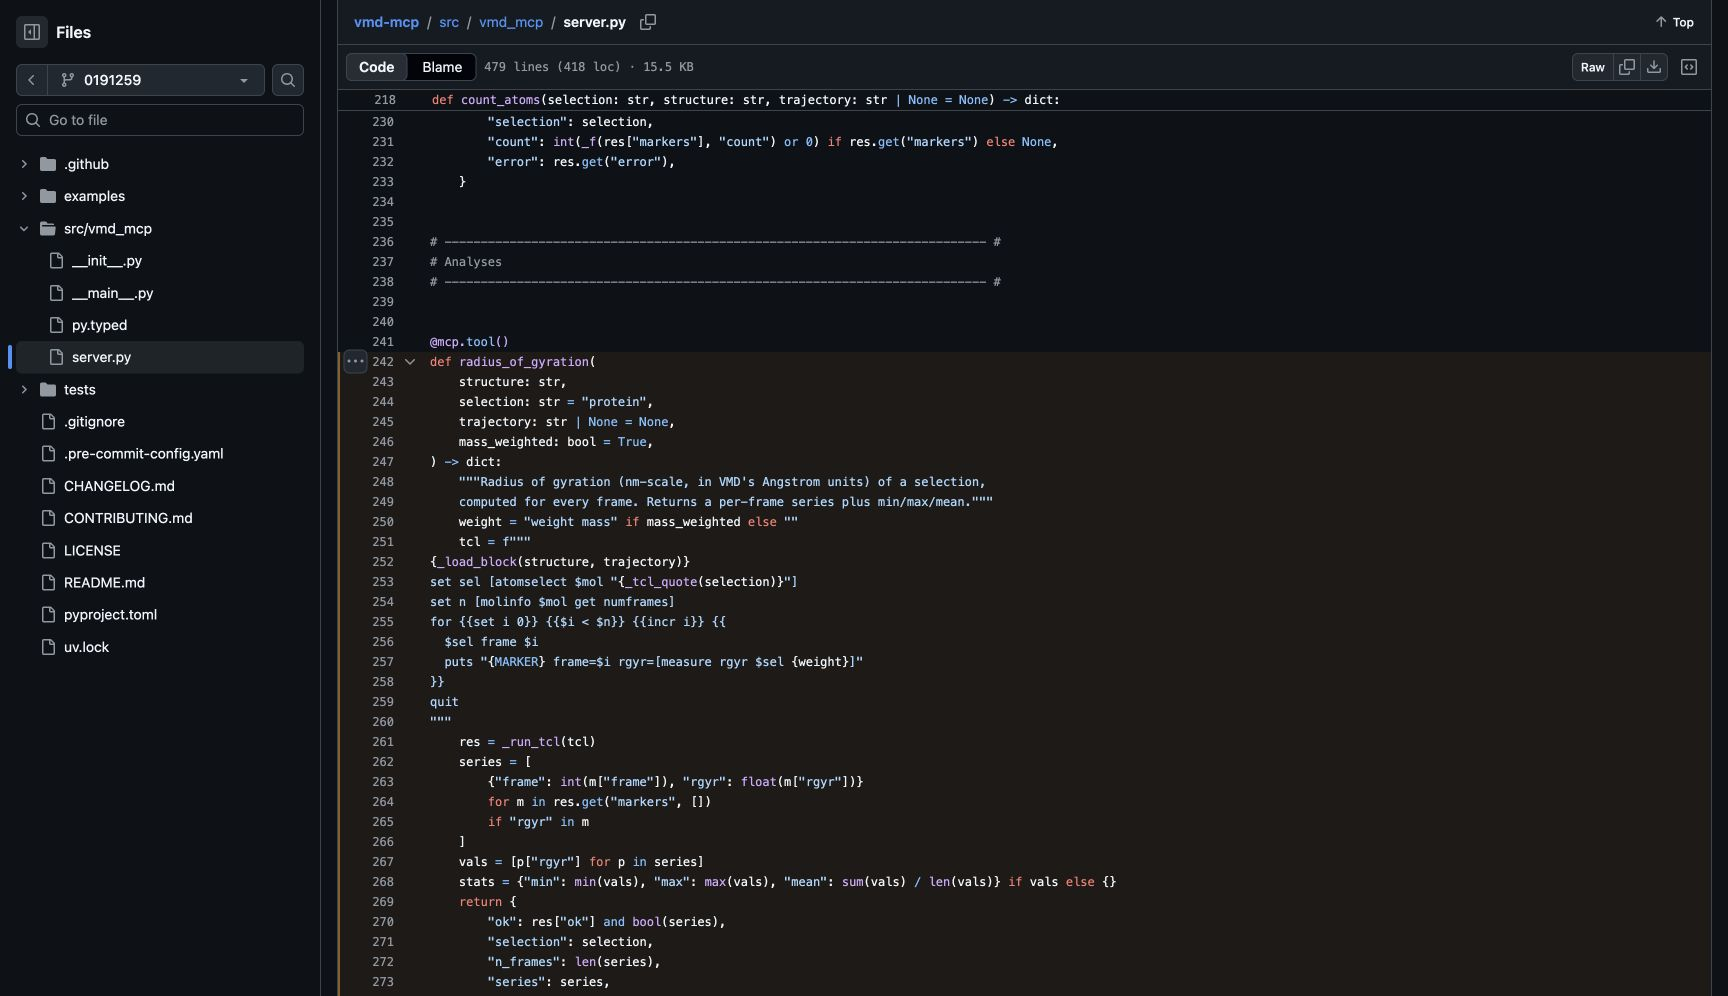
\includegraphics[width=.85\textwidth]{screenshots/vmd-gyration.jpg}
\caption{VMD MCP source at commit \texttt{0191259}: the gyration wrapper constructs a Tcl frame loop and parses marked values. The screenshot shows the repository tree, source path and real line numbers. The function's documented unit convention must be checked before comparison with other tools. \href{https://github.com/Alierkn/vmd-mcp/blob/01912595595bf0302124f57559e1e6a22095fb24/src/vmd_mcp/server.py\#L242-L278}{Open the inspected source}.}
\label{fig:vmdcode}
\end{figure}
\clearpage
\begin{codepanel}{03\quad Validate before starting a job}{GROMACS MCP / source lines 1452--1467}
\lstinputlisting[style=editorialcode,firstnumber=1452,gobble=8]{generated/gromacs-mcp-excerpt.py}
\end{codepanel}
\begin{figure}[htbp]
\centering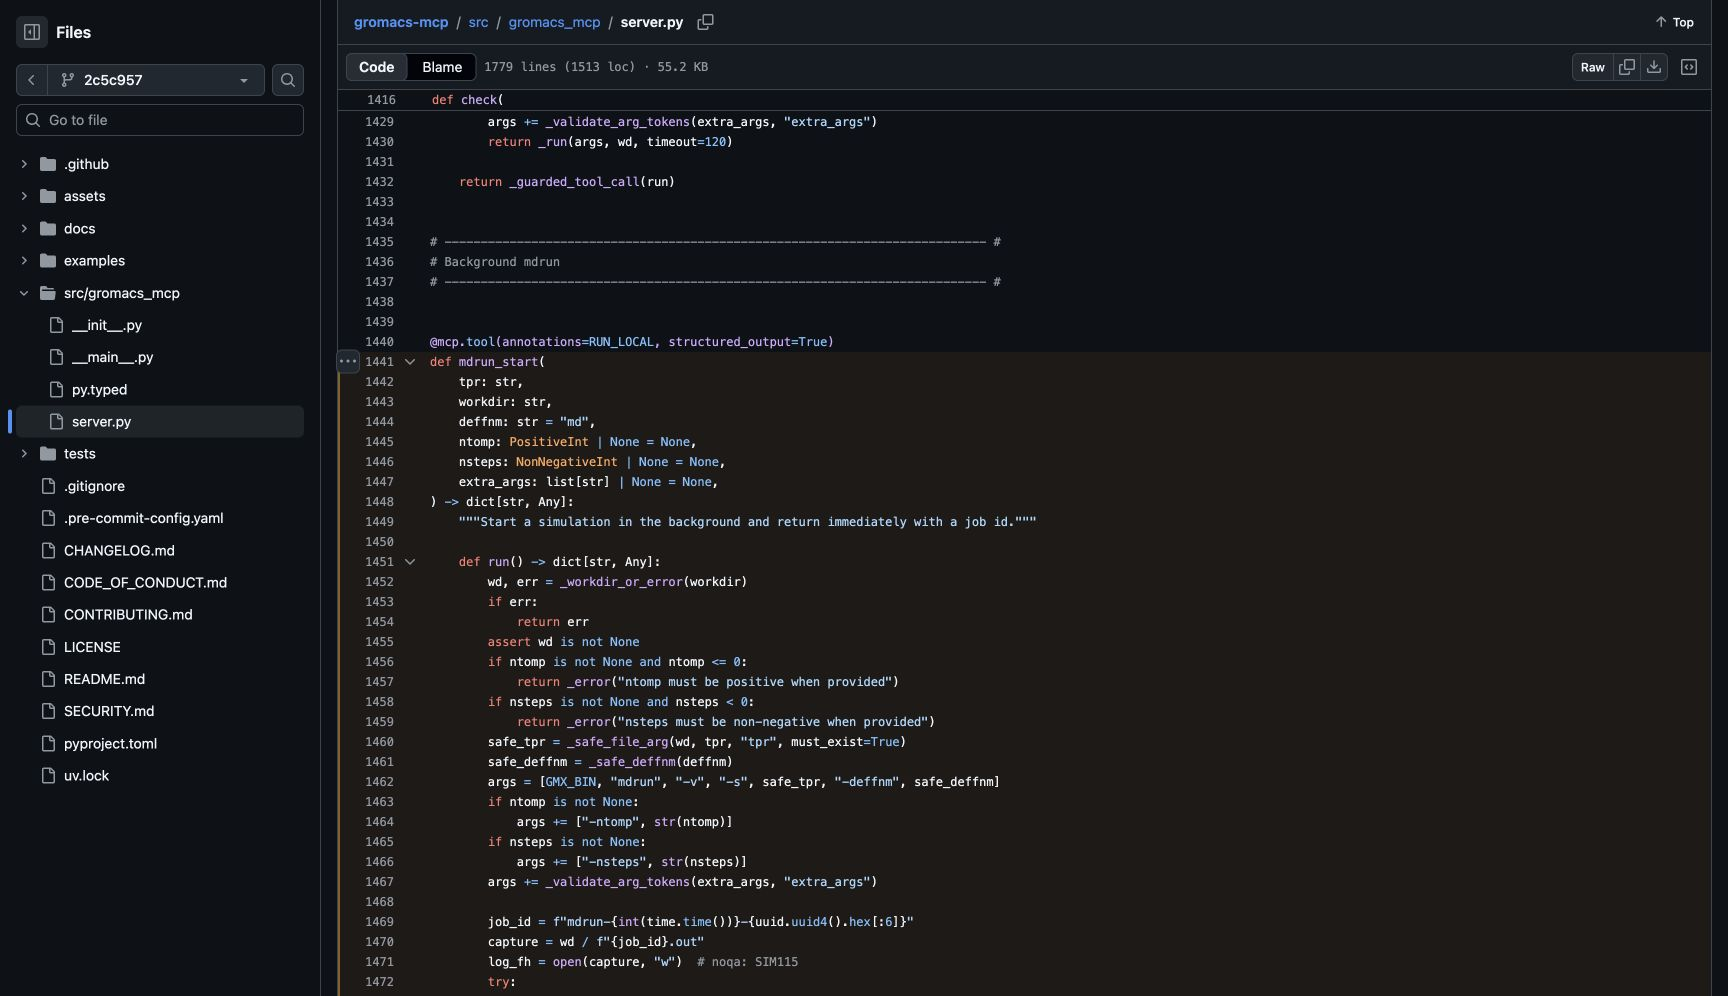
\includegraphics[width=.85\textwidth]{screenshots/gromacs-mdrun.jpg}
\caption{GROMACS MCP source at commit \texttt{2c5c957}: the background-run wrapper validates inputs, constructs the \texttt{mdrun} command and prepares an output log. This source view does not establish that an Aβ40 simulation was launched through the tool. \href{https://github.com/Alierkn/gromacs-mcp/blob/2c5c957c3f2c047888b63ae258ace3df34cb8773/src/gromacs_mcp/server.py\#L1441-L1479}{Open the inspected source}.}
\label{fig:gmxcode}
\end{figure}
